本节详述了编程语言包含内存模型的动机,并介绍了并行开发者应该熟悉的几个核心概念:\par

\begin{itemize}
	\item 数据竞争和同步
	\item 计算和内存栅栏
	\item 原子操作
	\item 内存序
\end{itemize}

要理解这些概念在C++、SYCL和DPC++中的表达和用法,就必须从高层次来考虑这些概念。具有丰富的并行编程经验,特别是使用C++的读者,可以跳过前面的内容。\par

\hspace*{\fill} \par %插入空行
\textbf{数据竞争和同步}

在程序中编写的操作不会直接映射到单个硬件指令或微操作。简单的加法操作,例如data[i] += x,可以分解成一系列的指令或微操作:\par

\begin{enumerate}
	\item 将data[i]加载到一个临时内存中(寄存器)。
	\item 计算将x添加到data[i]中。
	\item 将结果存储回data[i]。
\end{enumerate}

这不是我们在开发应用程序时需要担心的事情——添加的三个阶段将按照顺序执行,如图19-1所示。\par

\hspace*{\fill} \par %插入空行
图19-1 datai] += x的连续执行分为三个独立的操作
\begin{center}
	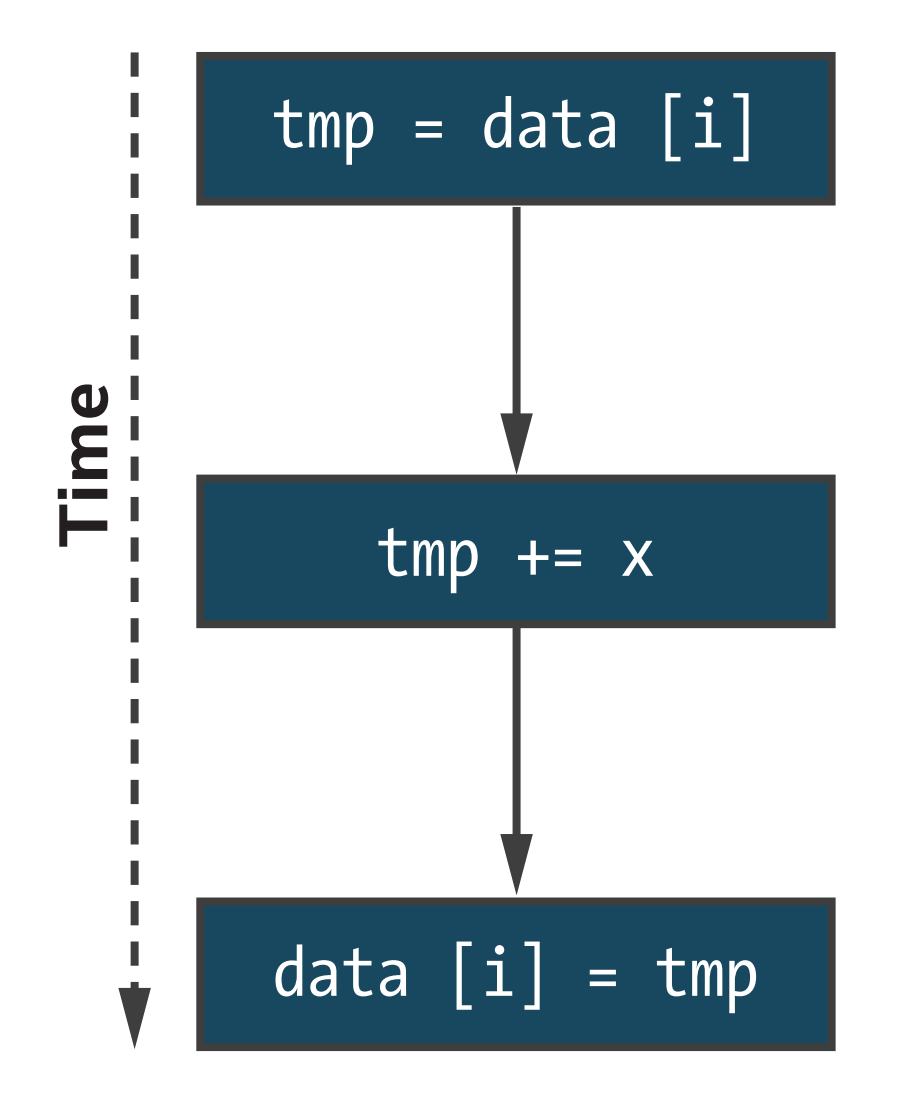
\includegraphics[width=1.0\textwidth]{content/chapter-19/images/2}
\end{center}

切换到并行应用程序开发带来了额外的复杂性:如果有多个操作同时应用于相同的数据,如何能确定对数据的一致性?考虑图19-2所示的情况,其中data[i] += x的两次执行交织在一起。如果两次执行,使用了不同的i值,则应用程序将正确执行。如果它们使用相同的i值,那会从内存中加载相同的值,并且其中一个结果会被另一个覆盖!这只是调度它们的操作的许多可能方式之一,应用程序的行为取决于哪个程序实例首先到达——这就是数据竞争。\par

\hspace*{\fill} \par %插入空行
图19-2 可能的data[i] += x交错并发执行
\begin{center}
	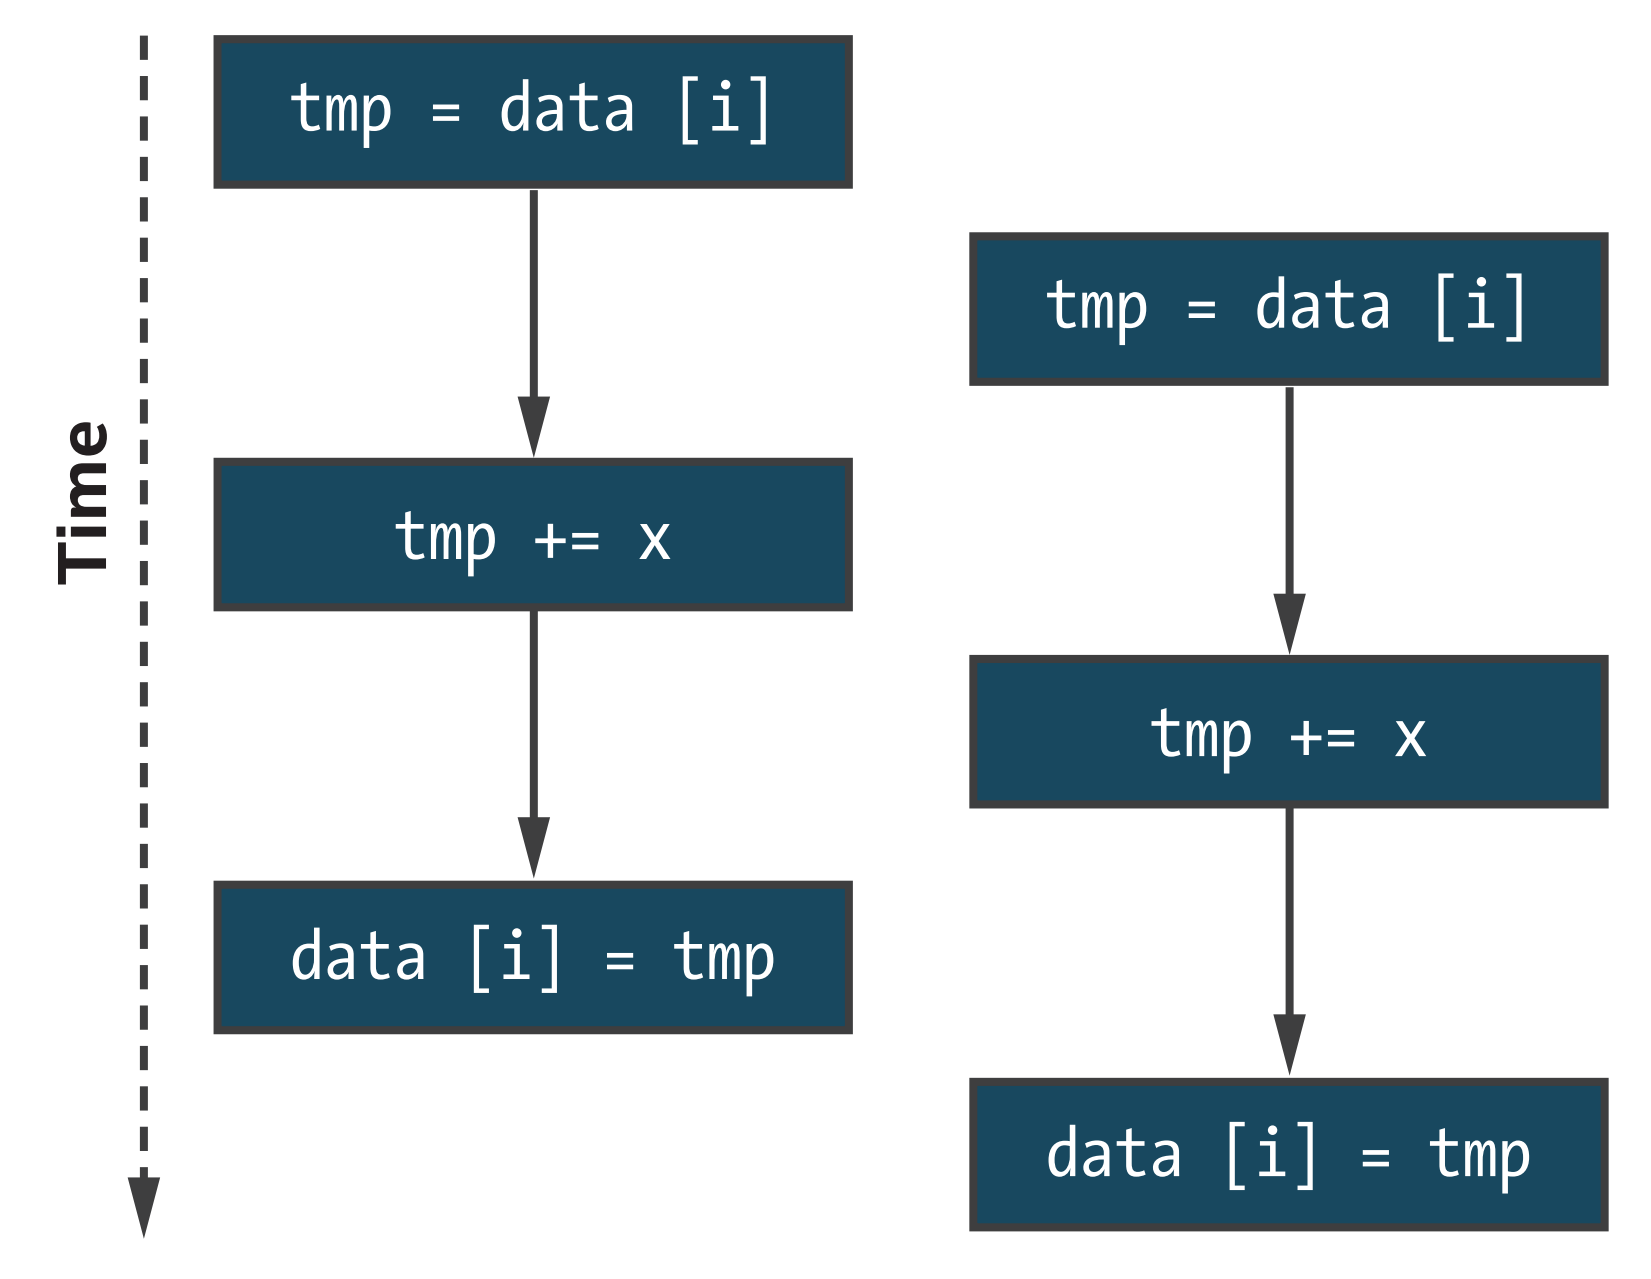
\includegraphics[width=1.0\textwidth]{content/chapter-19/images/3}
\end{center}

图19-3中的代码和图19-4中的输出展示了并发极易发生。如果M大于或等于N,则每个程序实例中j的值是唯一的;如果不是,j的值将会冲突,更新可能会丢失。我们说可能丢失是因为包含数据竞争的程序仍然可能在某个时间点,产生正确的答案(取决于实现和硬件如何安排工作)。无论编译器还是硬件都不可能知道这个程序要做什么,也不可能知道在运行时N和M的值是多少——作为开发者,有责任了解的程序是否包含数据竞争,以及是否对执行顺序敏感。\par

\hspace*{\fill} \par %插入空行
图19-3 包含数据竞争的内核
\begin{lstlisting}[caption={}]
int* data = malloc_shared<int>(N, Q);
std::fill(data, data + N, 0);

Q.parallel_for(N, [=](id<1> i) {
	int j = i % M;
	data[j] += 1;
}).wait();

for (int i = 0; i < N; ++i) {
	std::cout << "data [" << i << "] = " << data[i] << "\n";
}
\end{lstlisting}

\hspace*{\fill} \par %插入空行
图19-4 图19-3中的代码输出示例,用于小值N和M
\begin{tcolorbox}[colback=white,colframe=black]
N = 2, M = 2:\\
data [0] = 1\\
data [1] = 1\\
\\
N = 2, M = 1:\\
data [0] = 1\\
data [1] = 0
\end{tcolorbox}

通常,开发大规模并行应用程序时,不应该关注单个工作项执行的确切顺序——可能有数百(或数千!)个工作项同时执行,而特定的顺序将对可扩展性和性能产生负面影响。相反,我们的重点应该是开发可移植的正确执行的应用程序,可以通过向编译器(和硬件)提供关于程序实例何时共享数据、共享发生时,需要什么保证,以及哪些执行顺序是合法的信息来实现这一点。\par

\begin{tcolorbox}[colback=red!5!white,colframe=red!75!black]
大规模并行应用程序不应该关注单个工作项执行的确切顺序!
\end{tcolorbox}

\hspace*{\fill} \par %插入空行
\textbf{计算和内存栅栏}

防止同一组中工作项之间的数据竞争的一种方法是,使用工作组栅栏和适当的内存栅栏在不同程序实例之间引入同步。可以使用工作组栅栏对数据[i]的更新进行排序,如图19-5所示,图19-6给出了示例内核的更新版本。请注意,因为工作组栅栏不会同步不同组中的工作项,所以只有当我们将自己限制在单个工作组中时,示例才能保证正确执行!\par

\hspace*{\fill} \par %插入空行
图19-5 data[i] += x的两个实例被栅栏隔开
\begin{center}
	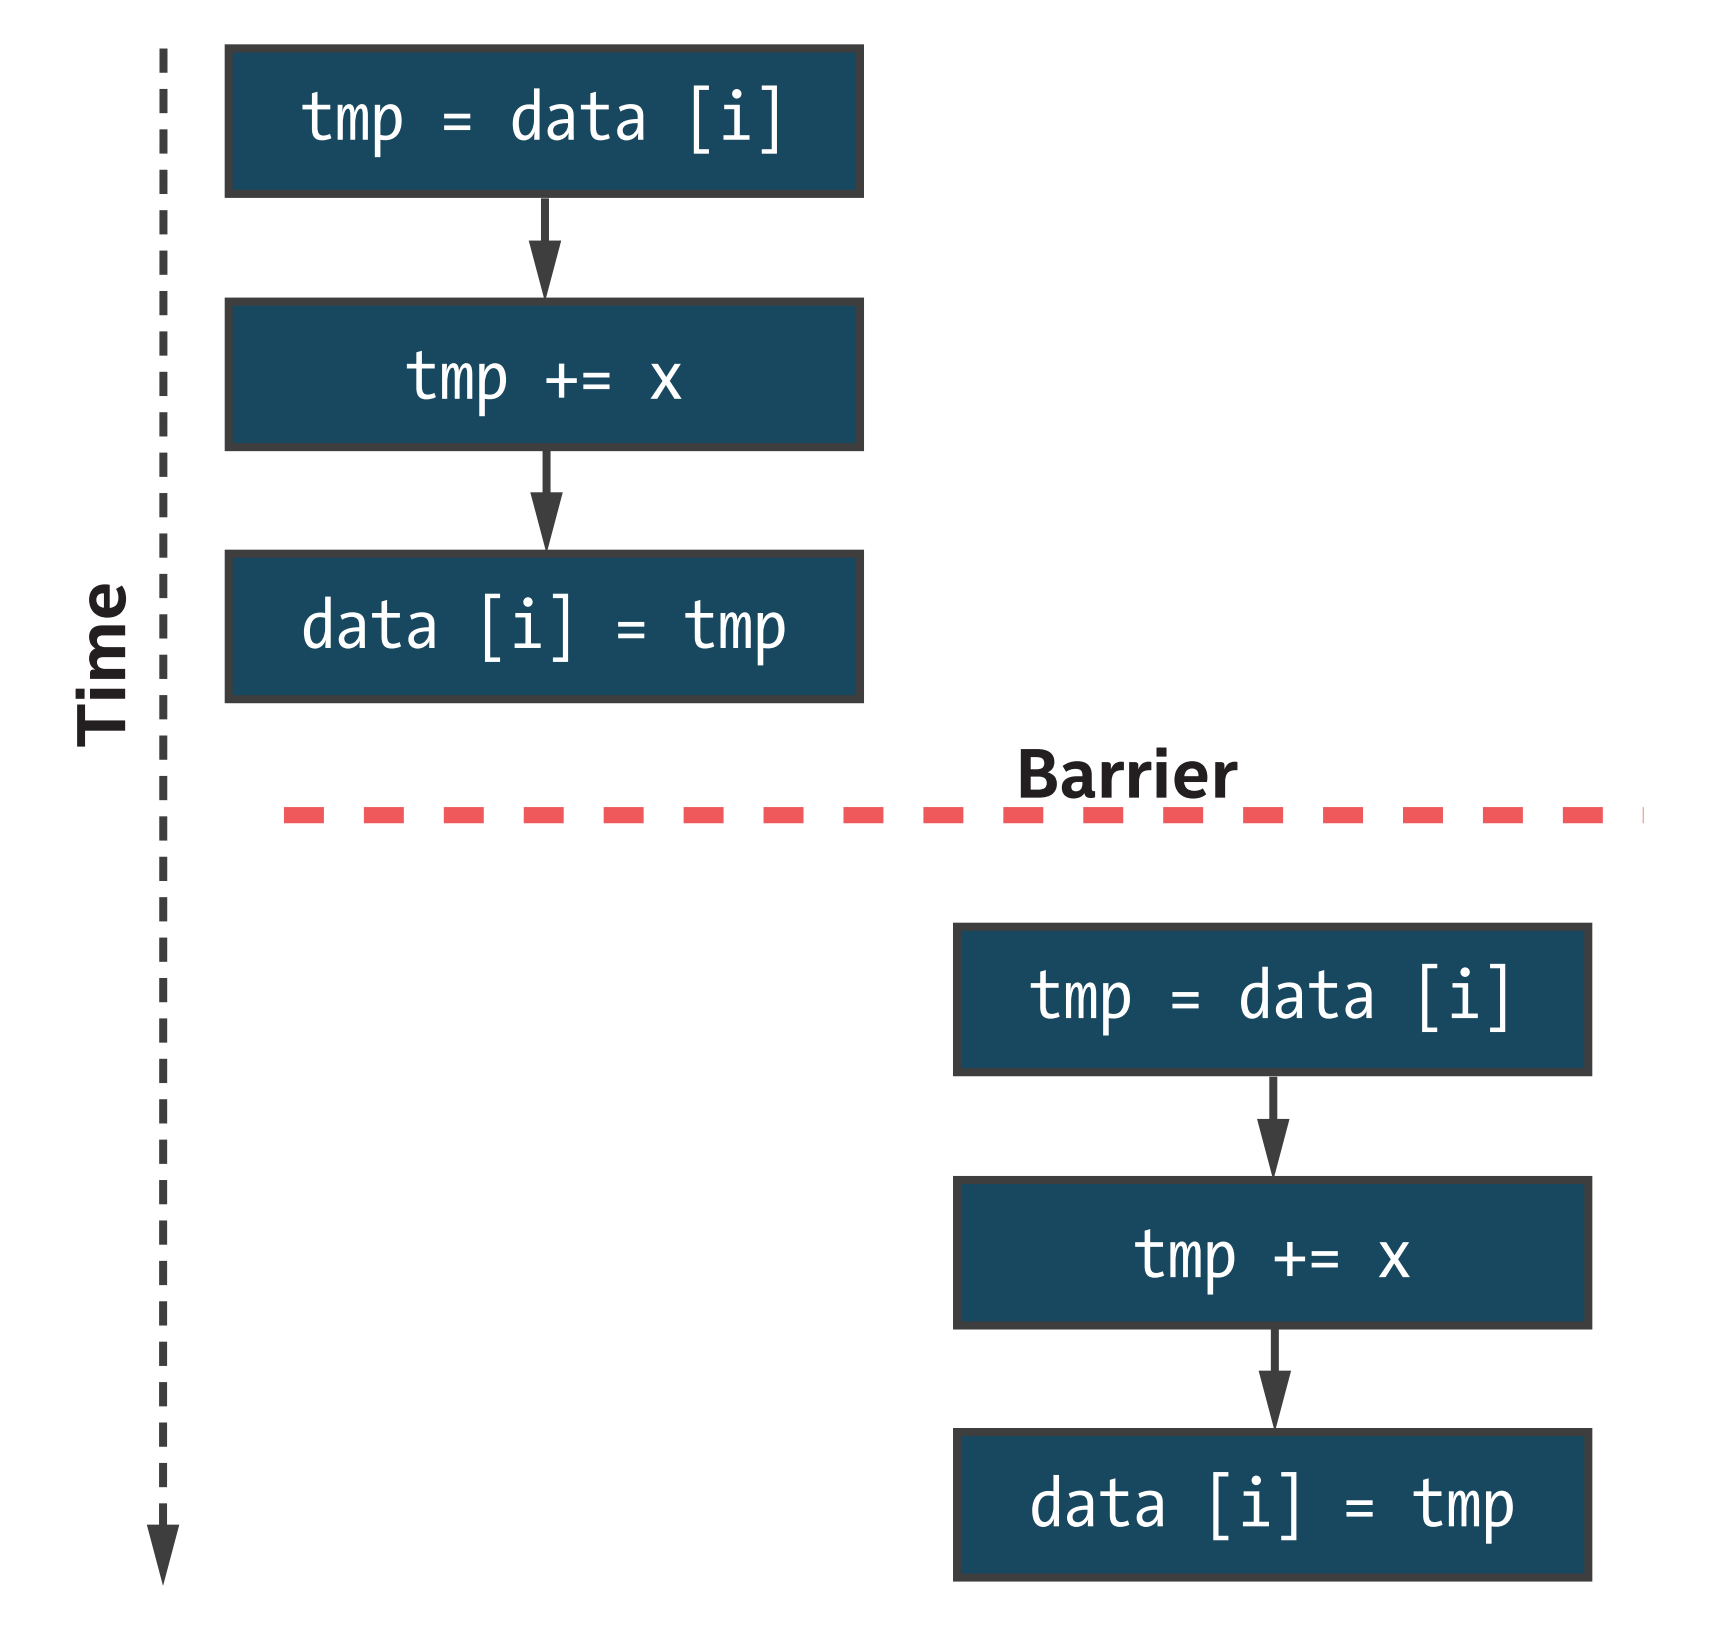
\includegraphics[width=1.0\textwidth]{content/chapter-19/images/4}
\end{center}

\hspace*{\fill} \par %插入空行
图19-6 使用障碍避免数据竞争
\begin{lstlisting}[caption={}]
int* data = malloc_shared<int>(N, Q);
std::fill(data, data + N, 0);

// Launch exactly one work-group
// Number of work-groups = global / local
range<1> global{N};
range<1> local{N};

Q.parallel_for(nd_range<1>{global, local}, [=](nd_item<1> it) {
	int i = it.get_global_id(0);
	int j = i % M;
	for (int round = 0; round < N; ++round) {
		// Allow exactly one work-item update per round
		if (i == round) {
			data[j] += 1;
		}
		it.barrier();
	}
}).wait();

for (int i = 0; i < N; ++i) {
	std::cout << "data [" << i << "] = " << data[i] << "\n";
}
\end{lstlisting}

尽管使用障碍来实现此模式没什么问题,但通常不鼓励这样做——它强制组中的工作项按顺序和特定的顺序执行,这可能导致负载不平衡的情况下长时间的不活动。它还可能引入比严格要求更多的同步——如果不同的程序实例碰巧使用了不同的i值,它们仍将在计算栅栏上进行同步。\par

栅栏同步是一种有用的工具,确保工作组或子工作组中的所有工作项在进入下一个阶段之前完成内核的某部分,但是对于细粒度的(可能依赖于数据的)同步来说,栅栏同步过重了。对于更通用的同步模式,我们必须使用原子操作。\par

\hspace*{\fill} \par %插入空行
\textbf{原子操作}

原子操作允许在不引入数据竞争的情况下并发访问内存位置。当多个原子操作访问同一内存时,保证它们不会重叠。如果只有一些访问具有原子性,那么这个保证就没意义,开发者有责任确保不会使用具有不同原子性的操作,去并发访问相同的数据。\par

\begin{tcolorbox}[colback=red!5!white,colframe=red!75!black]
同一个内存位置同时混合原子和非原子操作会导致未定义的行为!
\end{tcolorbox}

如果使用原子操作来表示简单的加法,结果可能如图19-8所示——每个更新都是不可分割的工作块,并且应用程序将总是产生正确的结果。对应的代码如图19-7所示——在本章后面重新讨论atomic\_ref类及其模板参数的含义。\par

\hspace*{\fill} \par %插入空行
图19-7 使用原子操作避免数据竞争
\begin{lstlisting}[caption={}]
int* data = malloc_shared<int>(N, Q);
std::fill(data, data + N, 0);

Q.parallel_for(N, [=](id<1> i) {
	int j = i % M;
	atomic_ref<int, memory_order::relaxed, memory_scope::system,
			   access::address_space::global_space> atomic_data(data[j]);
	atomic_data += 1;
}).wait();

for (int i = 0; i < N; ++i) {
	std::cout << "data [" << i << "] = " << data[i] << "\n";
}
\end{lstlisting}

\hspace*{\fill} \par %插入空行
图19-8 与原子操作交错执行的data[i] += x
\begin{center}
	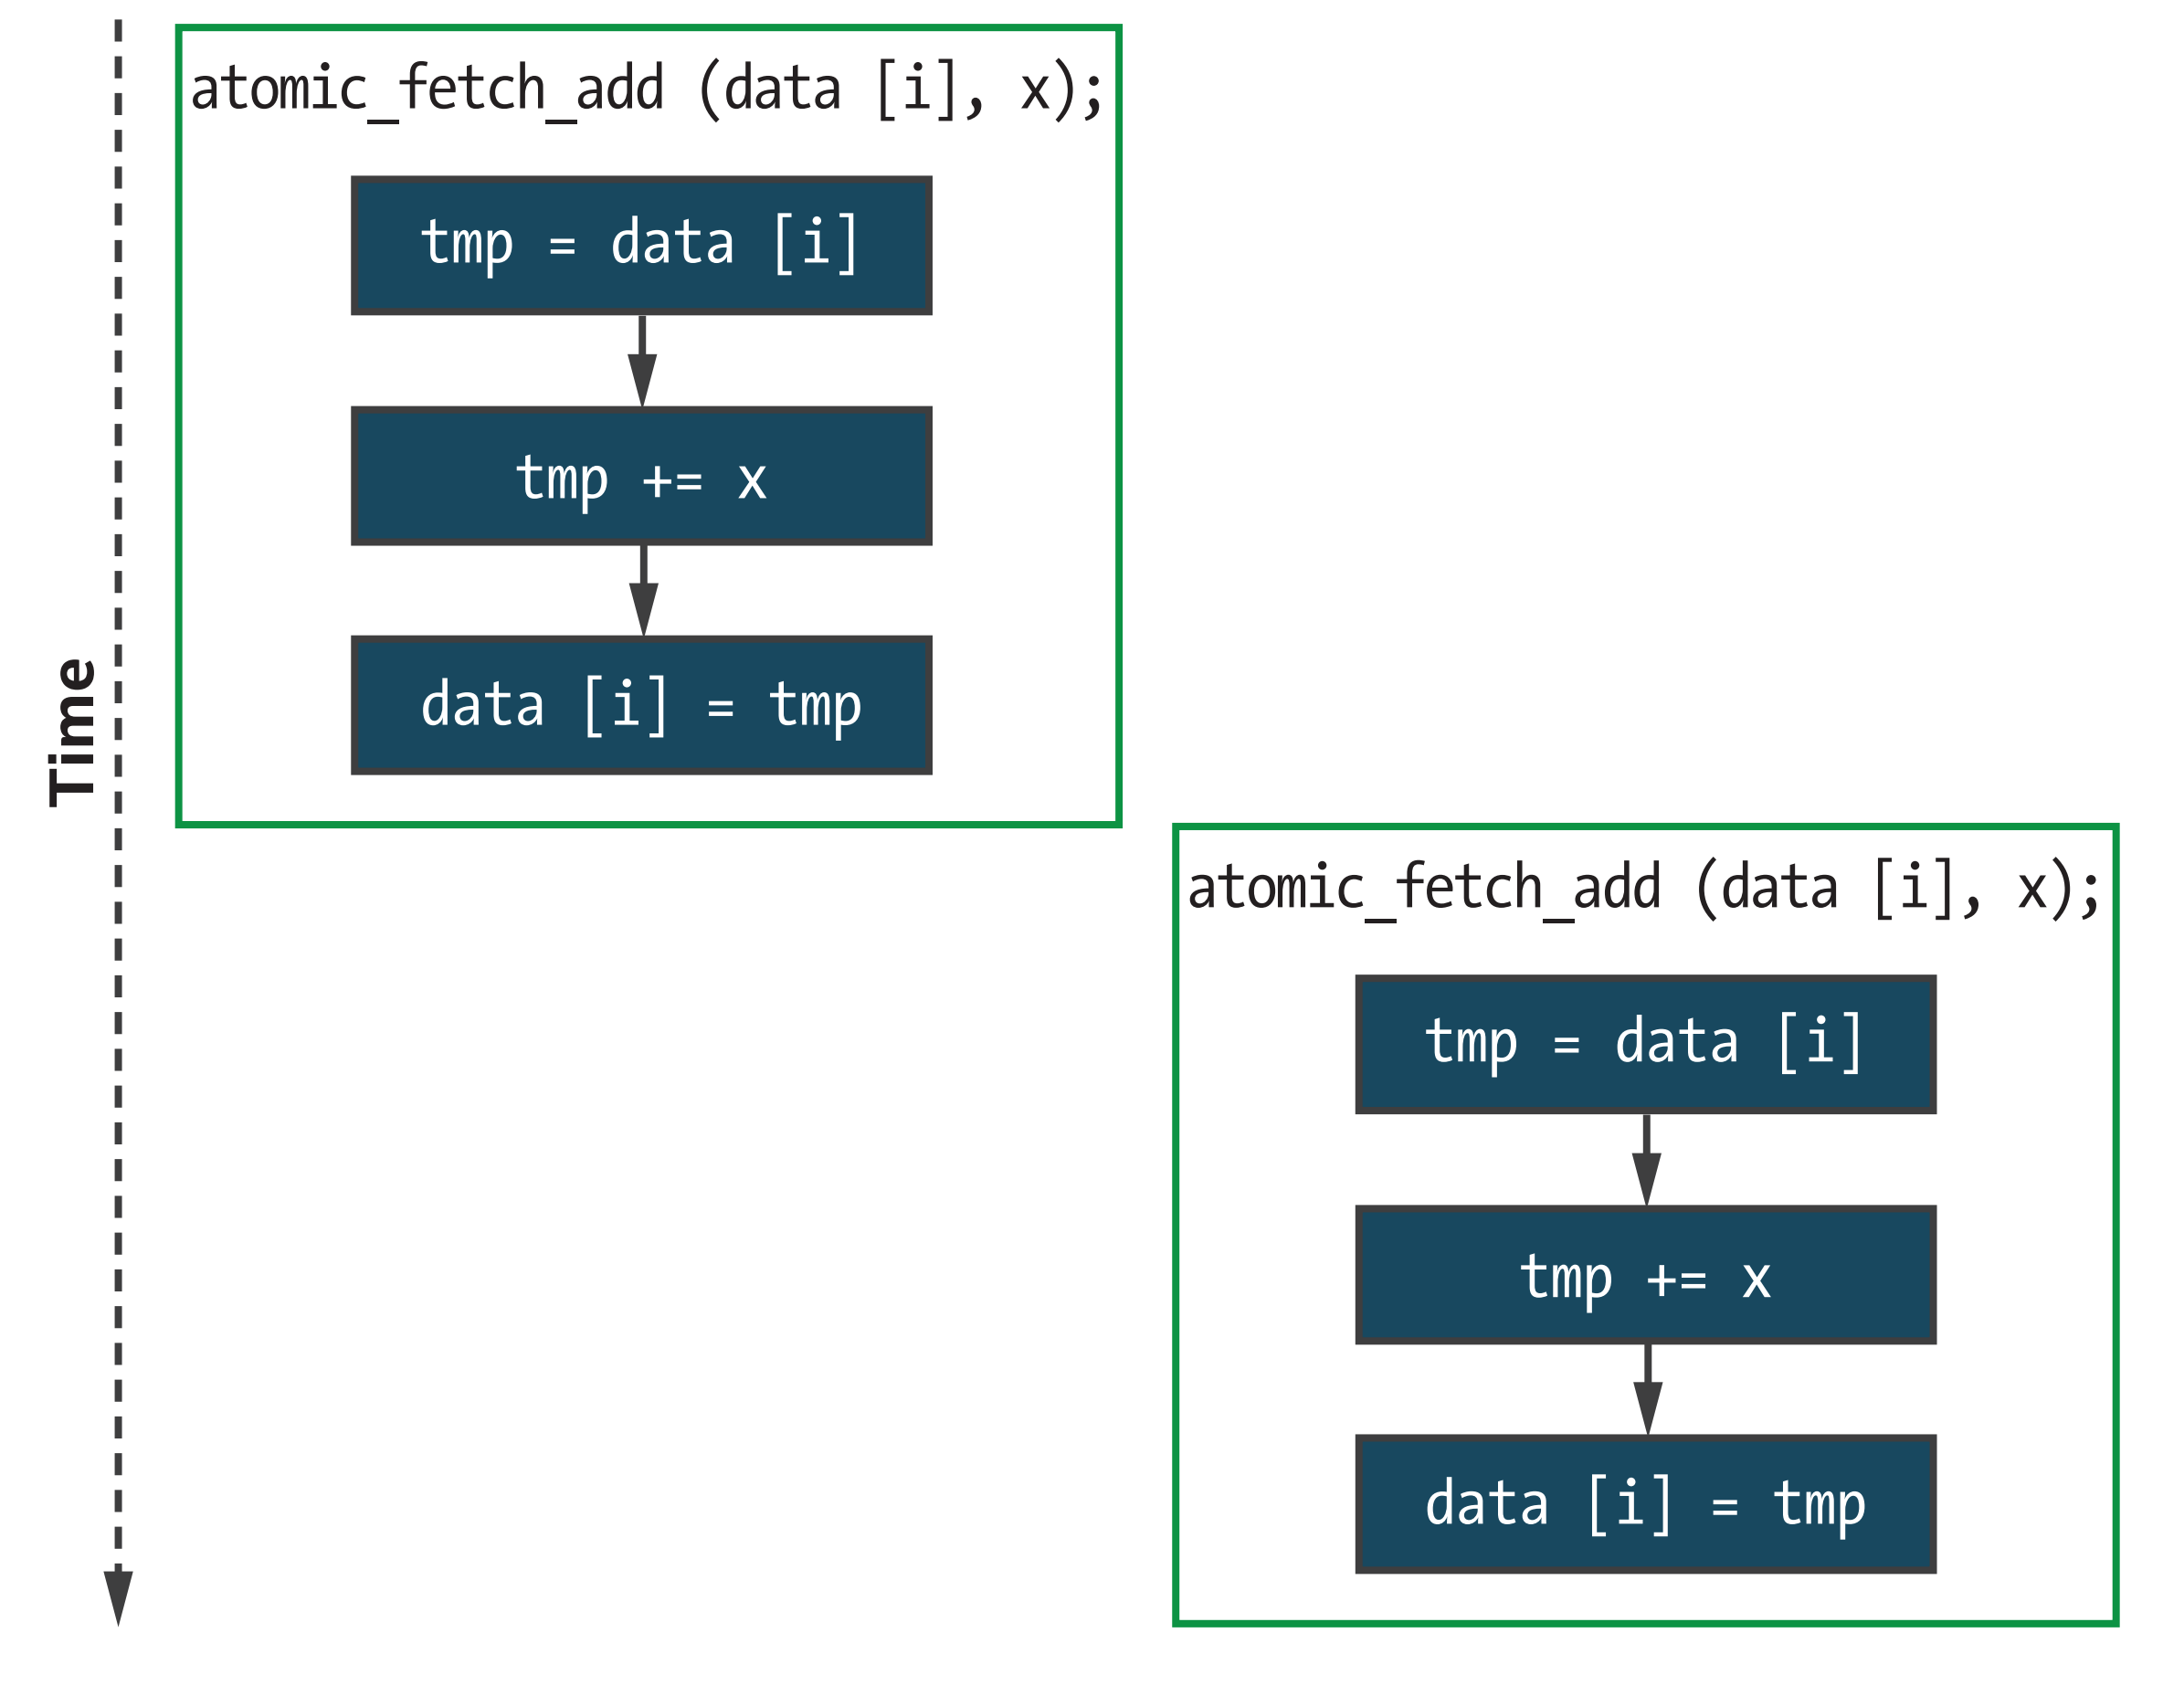
\includegraphics[width=1.0\textwidth]{content/chapter-19/images/5}
\end{center}

需要注意的是,这仍然只是一个\textbf{可能}的执行顺序。使用原子操作可以保证两个更新不重叠(如果两个实例使用相同的i值),但是不能保证两个实例中哪一个会先执行。更重要的是,不能保证这些原子操作相对于不同程序实例中的任何非原子操作的执行顺序。\par

\hspace*{\fill} \par %插入空行
\textbf{内存序}

即使在顺序应用程序中,优化编译器和硬件可以自由地重新排序操作。换句话说,应用程序的行为必须与开发者编写的程序完全一样。\par

然而,这种假设还不足以推断并行程序的执行。现在有两个需要担心的重排来源:编译器和硬件可能会在每个顺序的程序实例中重新排序语句的执行,而程序实例本身可能以任何(可能是交错的)顺序执行。为了设计和实现程序实例之间的安全通信协议,需要能够约束这种重新排序。为编译器提供我们想要的内存顺序的信息,可以防止与我们的应用程序的预期行为不兼容的重排优化。\par

有三种常用的内存顺序\par

\begin{enumerate}
	\item 自由的内存序
	\item 获取-释放或释放-获取的内存序
	\item 顺序一致的内存序
\end{enumerate}

在自由内存排序下,内存操作可以不受任何限制地重排。自由内存模型最常见的用法是增加共享变量(例如,一个计数器,直方图计算期间的一个值数组)。\par

获取-释放内存顺序下,程序实例释放一个原子变量,而另一个程序实例获取同一个原子变量,这两个程序实例充当同步点,并保证释放实例之前对内存的任何写操作对获取实例可见。通常,可以考虑原子操作将其他内存操作释放到其他程序实例,或者获取其他程序实例的内存操作。如果想通过内存在程序实例对之间传递值,就需要一个内存模型,这可能比想象的更常见。当程序获得锁时,通常会执行一些额外的计算,并在最终释放锁之前修改内存——只有锁变量会自动更新,但是我们希望由锁保护的内存更新能够避免数据竞争。这种行为依赖于获取-释放内存排序来保证,尝试使用自由内存序来实现锁是不行的。\par

顺序一致的内存顺序下,获取-释放顺序仍然有效,但所有原子操作的全局顺序一致。这种内存序行为是这三种方法中最直观的,也是最接近开发顺序应用程序时的习惯。有了顺序一致性,对程序实例组(而不是成对)之间的通信进行推理就会变得容易得多。\par

设计可移植的并行应用程序时,必须了解编程模型和设备的组合支持哪些内存顺序。明确地描述应用程序所需的内存序,可以确保当需要的行为不受支持时,可以预见地失败(例如,在编译时),并避免做出不安全的假设。\par







































